\documentclass[conference]{IEEEtran}
\IEEEoverridecommandlockouts
% The preceding line is only needed to identify funding in the first footnote. If that is unneeded, please comment it out.
%Template version as of 6/27/2024

\usepackage{cite}
\usepackage{amsmath,amssymb,amsfonts}
\usepackage{algorithmic}
\usepackage{graphicx}
\usepackage{textcomp}
\usepackage{xcolor}
\def\BibTeX{{\rm B\kern-.05em{\sc i\kern-.025em b}\kern-.08em
    T\kern-.1667em\lower.7ex\hbox{E}\kern-.125emX}}
\begin{document}

\title{Imitating Human Gestures for Social Interaction: Physical Greetings, Gesture Recognition, and Imitation with the UR5\\
}


\author{\IEEEauthorblockN{Jonah Blackmon}
\IEEEauthorblockA{
\textit{Living with Robots Laboratory} \\
\textit{University of Texas at Austin}\\
Austin, TX, USA \\
JonahKBlackmon@gmail.com}
\and
\IEEEauthorblockN{Lucas Helms}
\IEEEauthorblockA{
\textit{Living with Robots Laboratory} \\
\textit{University of Texas at Austin}\\
Austin, TX, USA \\
lucas.ray.helms@gmail.com}
}

\maketitle

\section{Introduction}
Human-robot interaction (HRI) is becoming increasingly prevalent in both industrial and non-industrial settings. However, a critical aspect of social interaction, non-verbal communication, is often underrepresented in current robotic systems. This limitation is particularly evident in existing research, where most non-verbal robots are typically tested in controlled environments, such as laboratories, where the focus is on interaction with the robot itself, rather than on natural interactions in real-world work environments or socially dynamic spaces. To address this gap, we developed a foundational system utilizing a network of ROS2 packages designed to support gesture recognition, real-time imitation, and a flexible framework that accommodates a wide range of programmable movements. We evaluated the system in three primary ways. First, we conducted an experiment in which participants were prompted to greet the robot, then assessed how approachable it was with and without the greeting implementation through a post-interaction survey. Second, we observed interactions with the robot in a natural setting, without any prompting, to evaluate if participants would instinctively engage with the robot, something typical of real-world work environments. Finally, we evaluated the system by testing its ability to detect and respond to gestures in real-time. These evaluations provide valuable insights into the potential for enhancing the social awareness and approachability of robots in dynamic, human-centered environments, as well as the broader need for robots to understand and communicate non-verbally in a socially aware manner.


\section{Related Work}
The demand for gesticulation in robots has been prevalent over the course of the last decade and even more so now. Even as early as 2006 research was being done on how humanoid robots can learn and replicate social cues, as demonstrated by Calinon and Billard, who trained a humanoid robot by physically positioning it to help it learn the desired gestures \cite{10.1145/1228716.1228751}. The emphasis on gesticulation of humanoid robots specifically supports the understanding that non-verbal communication aids in humans finding a robot more socially acceptable. We have also been able to learn that real-time gesture imitation has a positive effect on participants that interact with it. This is most clearly seen through an experiment run by Burns, Jeon, and Park in which a robot imitated participants in real-time, and the robot was found to be more socially accepted after it replicated participants' gestures \cite{app8020241}. These two experiments highlight the need for gesticulation in humanoid robots, however we want to find out if the support for gestures and mimicry in robots whose sole purpose is not social interaction will improve how comfortable participants may be working alongside these robots. While much of the early research into robot gestures has centered on humanoid robots designed for social interaction, there is growing interest in exploring how gesticulation can be beneficial for non-social robots—robots that are not explicitly intended to interact socially, but are tasked with performing practical roles. A notable example is found in the medical field, where non-humanoid robotic assistants are becoming more prevalent. In a study conducted by Tiferes and Hussein \cite{article}, it was found that up to 66 percent of communication during surgeries was non-verbal, underscoring the importance of non-verbal cues in high-stakes environments. This finding highlights the need for robots working in such environments to communicate effectively using gestures, despite not being primarily designed for social interaction. These studies demonstrate the potential for non-social robots, particularly those working alongside humans in settings such as healthcare, to benefit from incorporating gesticulation and other forms of non-verbal communication to improve collaboration and efficiency.
\section{Method}
To enable gesticulation and social responsiveness in the V5-BWI Bot, we developed a system composed of multiple ROS2 packages. The system consists of two main functional modules: gesture-based greeting recognition and real-time gesture imitation. The greeting functionality is achieved through two coordinated ROS2 nodes. The first node processes a live camera feed using MediaPipe to identify human hands within the image. Once hands are detected, the system segments the palm from the fingers and determines whether the palm is open, which is used as a heuristic for detecting a wave. If an open palm is consistently identified across a series of frames, a signal indicating the presence of a greeting gesture is published. While this implementation targets a simple wave gesture, the modular structure of the detection pipeline allows for future expansion to more complex hand gestures. The second node is responsible for controlling the UR5 robotic arm's dynamic motion. It subscribes to the output from the gesture recognition node and initiates a movement from its initial state to its goal state, in this example, a greeting motion, only while a user is actively waving at it. The arm returns to its default position when the wave ceases. Rather than relying on hardcoded timings, the duration and smoothness of the movement are determined based on the spatial distance between joint configurations. This approach allows gestures of varying lengths and scales to execute fluidly, improving adaptability and extensibility. The second core module enables real-time imitation of user hand motions. A ROS2 package processes the camera feed to track hand landmarks and derive the trajectory of the user’s palm in three-dimensional space. This trajectory is then published to a separate node. By subscribing to the hand trajectory and adjusting our goal state accordingly, the system enables the robot to imitate user movements with minimal latency. Because this imitation mechanism is implemented using the same dynamic motion node as the greeting system, only the target pose generation logic differs. This reuse of infrastructure significantly streamlined development and highlights the generality of the proposed control framework. When integrated with the Universal Robots UR5 Driver, the system enables the robot to operate in a socially responsive manner, either by initiating a contextualized greeting or by performing real-time imitation. This modular design supports future enhancements such as additional gesture classes, more advanced motion planning, or multimodal interaction cues, thus providing a scalable foundation for socially aware robotic behavior.
\section{Experimental Setup}
This experiment was designed to evaluate whether the integration of a gesture-based greeting system influenced participants' perceptions of the V5-BWI Bot’s social approachability. We conducted two complementary studies. The first was a controlled survey-based assessment involving 16 undergraduate students from the University of Texas at Austin. Participants were asked to rate the robot’s approachability on a five-point scale, both based on their prior experiences with the standard BWI-Bot and following their interaction with the enhanced greeting implementation. This comparison allowed us to directly assess perceptual changes attributable to the system modification. Second, to examine spontaneous user engagement in a naturalistic setting, we deployed the V5-BWI Bot in the Living with Robots Laboratory during peak foot-traffic hours. The robot continuously executed the optional greeting behavior for one hour, accompanied by signage prompting interaction with the text “Wave at me!”. During this period, we used the same camera that detects the wave to record the space, enabling post-hoc analysis of human-robot interactions without direct prompting or experimental interference. This observational approach aimed to assess whether the presence of the greeting behavior influenced unprompted social engagement in a semi-public, organically populated environment. 
\section{Results}
Participants reported significantly increased perceptions of social approachability following the introduction of the greeting implementation. Prior to the implementation, the average participant rating for the V5-BWI Bot’s approachability was 1.65 out of 5 on a Likert scale. After interaction with the gesture-enabled system, this average rose to 4.65 out of 5. These results are illustrated in Figure 1, which presents a side-by-side comparison of the pre and post-implementation ratings.
\begin{figure}[!t]
\centering
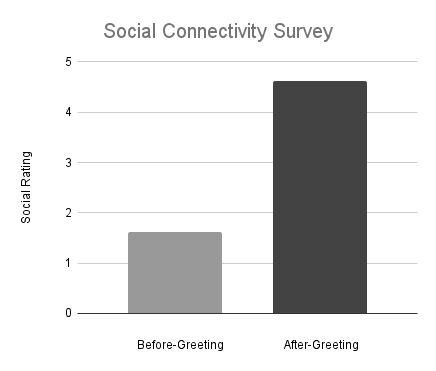
\includegraphics[width=\linewidth]{figures/Social Connectivity Survey.png}
\caption{Average participant ratings of robot approachability before and after the greeting implementation.}
\label{fig:Social Connectivity Survey}
\end{figure}
Qualitative feedback from participants supported these findings, with several describing the robot as "friendly" and "cute." In our unprompted observational study, we further noted a marked increase in spontaneous user interactions with the robot. Participants exhibited behaviors such as waving, sustained visual engagement, and even direct curiosity about the system itself—one individual attempted to access the robot’s terminal to learn more about its functionality. These results suggest that even minimal gestural capabilities can significantly enhance the perceived social presence of a robot, particularly in non-humanoid, industrial-style platforms. This finding supports the hypothesis that gesticulation and social signaling are not limited to anthropomorphic robots, but can play a meaningful role in improving human-robot interaction across a broader range of robotic systems.
\section{Discussion}
The results of our study suggest that even non-humanoid robots can benefit significantly from incorporating socially responsive behaviors. Participants rated the robot as notably more approachable when it performed a greeting gesture, indicating a clear human preference for social cues—even from function-focused machines. This highlights a growing demand for socially aware robotic systems across both industrial and non-industrial domains. The modular gesture recognition and imitation framework we developed lays a scalable foundation for future work in non-verbal robot communication. While our implementation focused on greeting and palm-based imitation, the underlying architecture supports a broader gesture vocabulary and real-time motion mapping. These capabilities can be extended to enable robots to complement verbal communication with expressive gestures. Potential applications include use in clinical settings, where both patients and healthcare professionals may feel more at ease around service robots capable of reading and responding to gestures. Similarly, gesture imitation could enhance collaborative manufacturing workflows, allowing robots to mirror human actions for intuitive teleoperation or training. Beyond immediate functionality, this work contributes to the broader effort of integrating non-verbal communication into robot design—not only for operational efficiency but also to improve social presence and human comfort. Future research should explore larger participant groups, extended gesture sets, and the integration of speech and gesture for multimodal interaction.
\section{Conclusion}
This work aimed to enhance social interaction between humans and robots by enabling gesture-based greetings and body language recognition. We developed a modular ROS2-based system for the V5-BWI robot that supports gesture detection, real-time imitation, and responsive motion control. Our user study demonstrated that the integration of a simple greeting gesture significantly improved participants’ perceptions of the robot, increasing its approachability and perceived personality. These findings underscore a growing expectation for social responsiveness even in non-humanoid, industrial-style robots. Furthermore, we discussed how this foundational system could be extended to domains such as healthcare and collaborative manufacturing. Overall, this work highlights the value and feasibility of integrating non-verbal communication into robotic systems to support more natural and effective human-robot interaction

\bibliographystyle{IEEEtran}
\bibliography{project}

\end{document}
